\documentclass{beamer}

\usetheme{Pittsburgh}
\usefonttheme[onlylarge]{structurebold}
\setbeamerfont*{frametitle}{size=\normalsize,series=\bfseries}
\setbeamertemplate{navigation symbols}{}

\usepackage{pdfpages}
\usepackage{soul}
\usepackage{ucs}

% encoding settings
%\usepackage[T2A]{fontenc}
\usepackage{xltxtra}
\usepackage{hyperref}
\usepackage{polyglossia}
%\usepackage{xecyr}
\usepackage{tikz}
\usepackage{listings}

\setdefaultlanguage{english}

% fonts settings
\usepackage{fontspec}
%\setmainfont{CMU Serif} % Computer Modern Unicode font
%\setsansfont{CMU Sans Serif}
%\setmonofont{CMU Typewriter Text}


\author[Author, Vladimir Shakhov]{Vladimir Shakhov \newline R\&D Senior Development Engineer }
\institute[Fujitsu Technology Solutions]
{
  Fujitsu Technology Solutions, R\&D department
}

\date[\now]

\lstset{language=bash,frame=single,}

\pgfdeclareimage[height=1.5cm]{fujitsu-logo}{logo/fujitsu-logo.png}
\pgfdeclareimage[height=3cm]{fujitsu-shaping}{fujitsu-shaping.jpg}
\pgfdeclareimage[height=5cm]{rx2560m1}{RX2560-M1.jpg}

\logo{\pgfuseimage{fujitsu-logo}}

\title{Linux firmware for iRMC controller on Fujitsu Primergy servers}



\begin{document}

\usebackgroundtemplate{%             declare it
\tikz[overlay,remember picture] \node[opacity=0.3, at=(current page.center)] {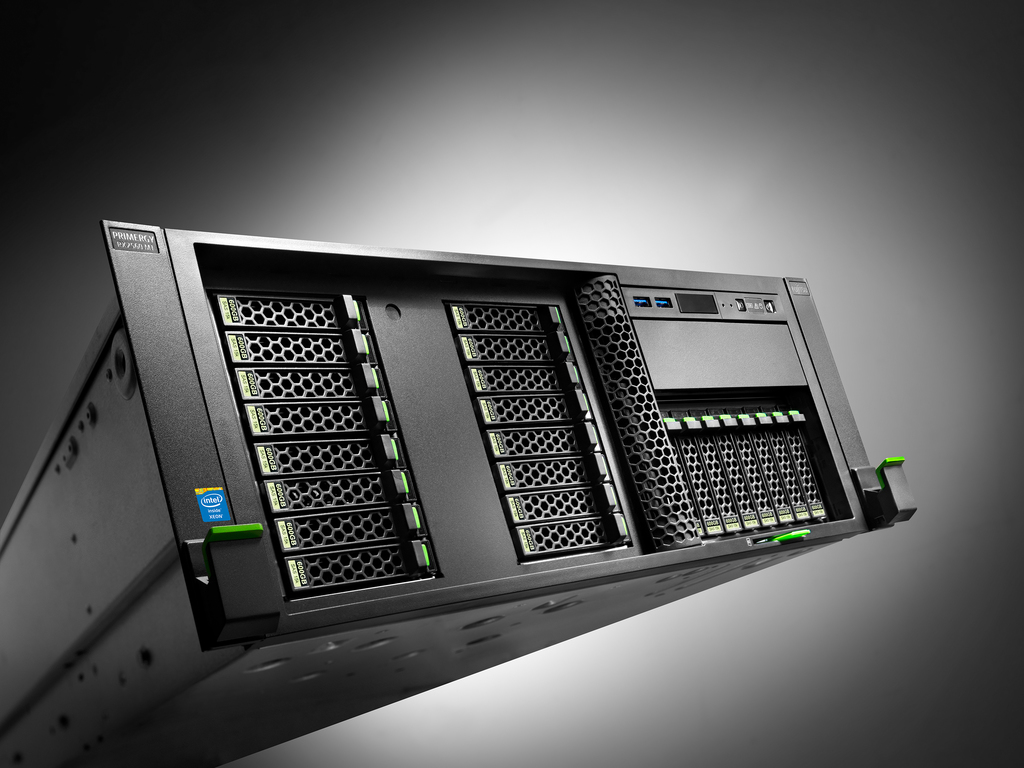
\includegraphics[height=\paperheight]{RX2560-M1.jpg}};
}

\begin{frame} 
  \titlepage 
\end{frame} 

\usebackgroundtemplate{} %unset

\begin{frame}{Table of content}
  \tableofcontents
  % You might wish to add the option [pausesections]
\end{frame}


\section{Fujitsu Primergy servers family}
	
  \subsection{What is iRMC}
  
  \begin{frame}{Fujitsu Primergy Servers}
	Lineage of x86-based servers: 
	
	Blade (BX), Rack (RX), Tower (TX) and Cloud (CX).
	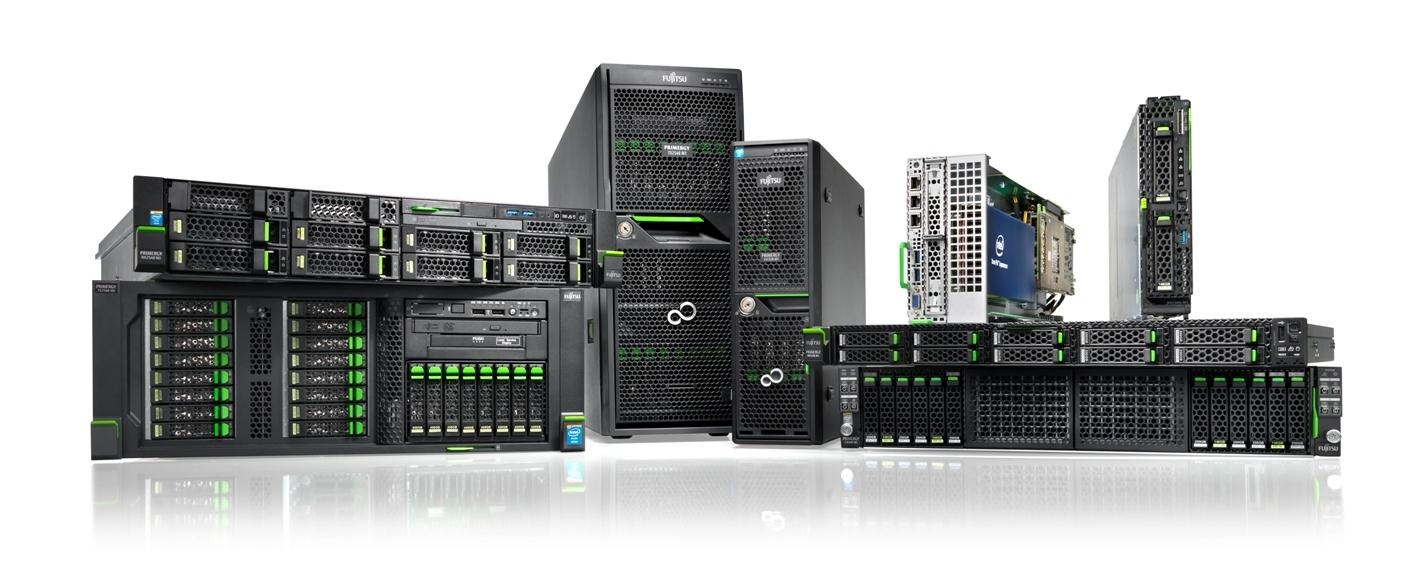
\includegraphics[scale=0.23]{primergy-servers.png}
  \end{frame}

  \begin{frame}{iRMC S4 in the wild}
	  \begin{center}
		  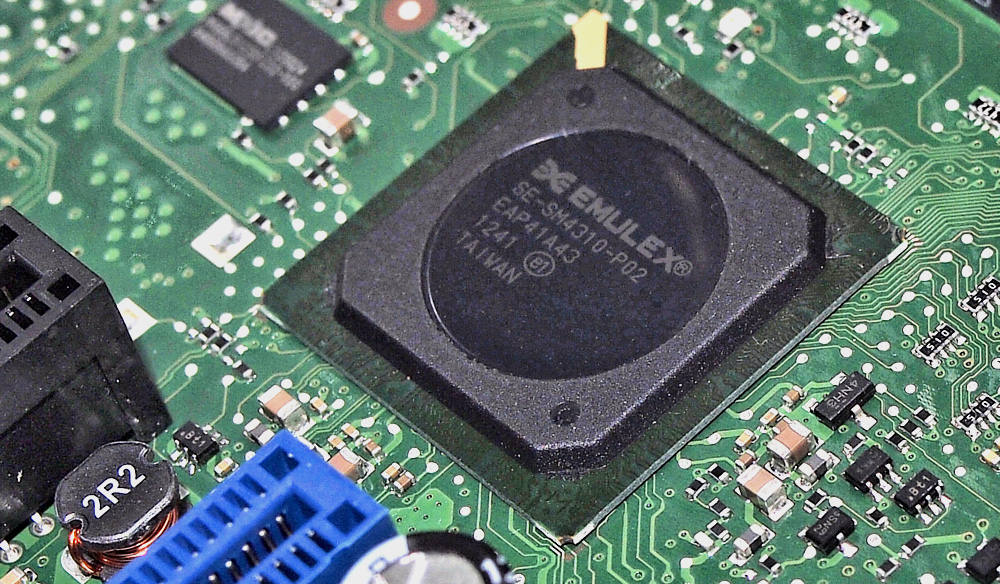
\includegraphics[scale=0.3]{irmc-s4-chip.png}
	  \end{center}
  \end{frame}

  \begin{frame}{iRMC - integrated Remote Management Controller}
	  \begin{block}{ARM-based SoC}
		  \begin{columns}[onlytextwidth]
			  \begin{column}{0.7\textwidth}

				  Emulex Pilot3 iBMC ASIC

				  Integrated BMC 

				  Super I/O

				  Graphics controller


			  \end{column}
			  \begin{column}{0.2\textwidth}
				  
\includegraphics[width=\textwidth]{logo/ARM_powered.png}
			  \end{column}
		  \end{columns}

		  KVMS: Remote Keyboard, Video, Mouse and Storage

		  CPU: 32-bit 400MHz ARM9 processor with MMU.
	  \end{block}
	  \pause

	  \begin{block}{Control x86 hardware}
		  Work independent if x86 host on or off.
	  \end{block}
	  \pause

	  \begin{block}{Own Operation System}
		  Very typical Embedded Linux.
	  \end{block}
	  
  \end{frame}

  \begin{frame}{iRMC basic features}
	  \begin{columns}[onlytextwidth]
  		  \begin{column}{0.6\textwidth}
			  \begin{itemize}
				  \item Web access (own web-server)
				  \item Security (SSL and SSH included)
				  \item ServerView suite Integration
				  \item Power management
				  \item SNMPv1/v2c/v3 support
				  \item Text console redirection
				  \item “Headless” system operation
				  \item CLP - command line interface 
			  \end{itemize}
		  \end{column}

  		  \begin{column}{0.4\textwidth}
			  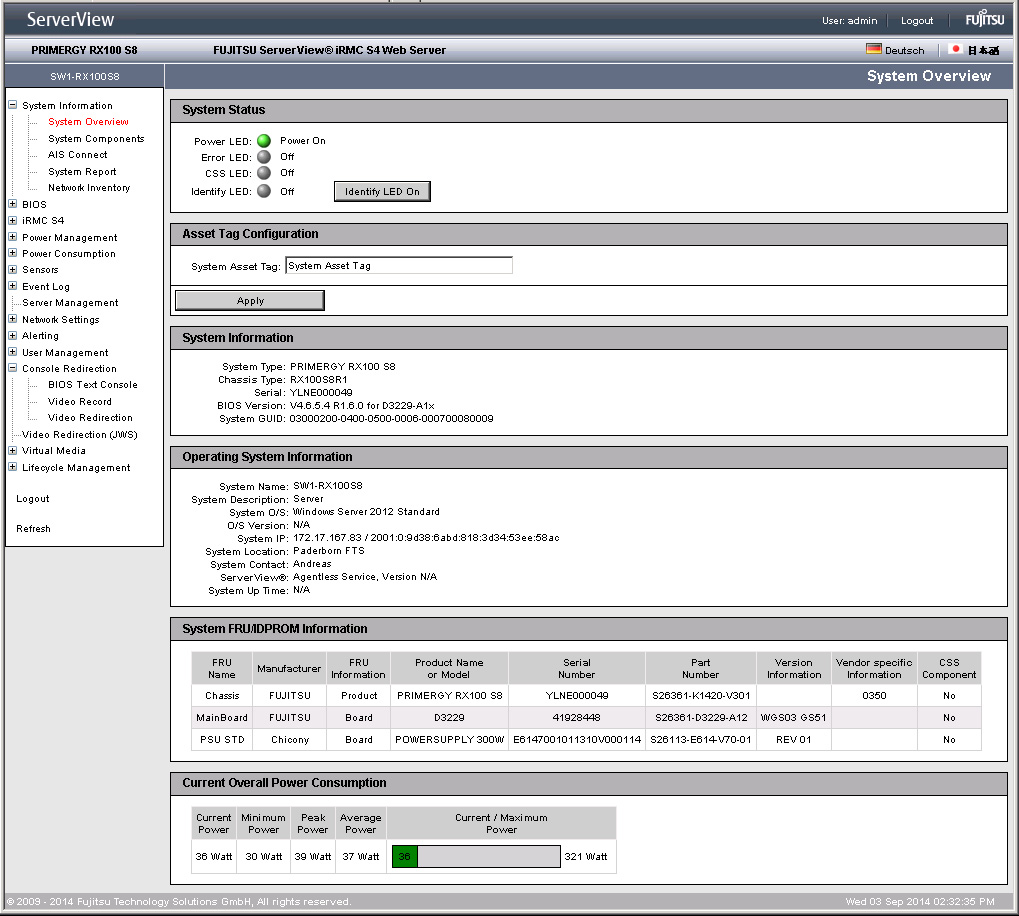
\includegraphics[width=\textwidth]{screenshot/webif.png}
		  \end{column}
	  \end{columns}

  \end{frame}

  \begin{frame}{iRMC advanced features}
	  \begin{itemize}
		  \item Advanced Video Redirection (AVR)
		  \item Virtual Media
		  \item Embedded Lifecycle Management (eLCM)
	  \end{itemize}
	  \begin{center}
		  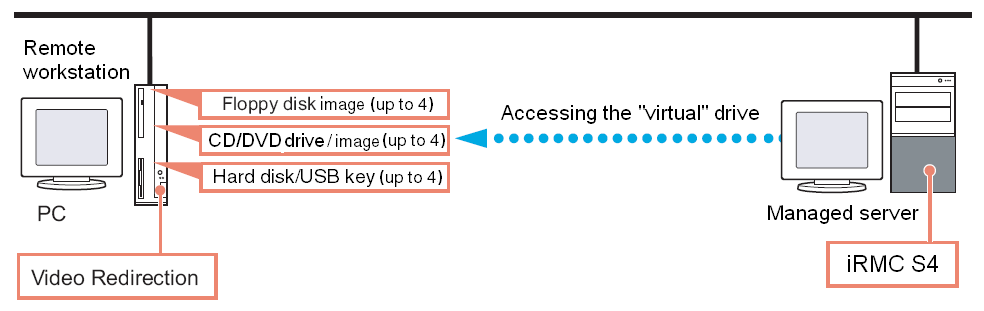
\includegraphics[width=0.9\textwidth]{diagrams/irmc-advanced-features.png}
	  \end{center}
  \end{frame}

  \subsection{Software - ServerView Suite}
  \subsection{ Open standards: IPMI protocol and others}
	\begin{frame}{Open standards}

		\begin{columns}[onlytextwidth]
			\begin{column}{0.2\textwidth}
				
\includegraphics[width=\textwidth]{logo/html.png}

				
\includegraphics[width=\textwidth]{logo/http.png}

				
\includegraphics[width=\textwidth]{logo/openssh.png}

				
\includegraphics[width=\textwidth]{logo/openssl.png}

				
\includegraphics[width=\textwidth]{logo/netsnmp.jpg}
			\end{column}

			\begin{column}{0.1\textwidth}
			\end{column}

			\begin{column}{0.7\textwidth}
			\begin{block}{Intelligent Platform Management Interface}
				IPMI - standardized, abstract, message-based interface between BMC and intelligent hardware for platform management.
				Key component of system.
			\end{block}
			\pause

			\begin{block}{Web: HTTP, HTML, JavaScript}
				Web-based control interface.
			\end{block}
			\pause

			\begin{block}{SNMP ver 1/2x/3}
				Popular protocol for network management.
			\end{block}
			\pause

			\begin{block}{Security: SSH and SSL}
			\end{block}
			\end{column}

		\end{columns}
	\end{frame}
  
   \subsection{iRMC internals}
   \begin{frame}{IPMI  - key interface of a system}
   	   \begin{center}
		   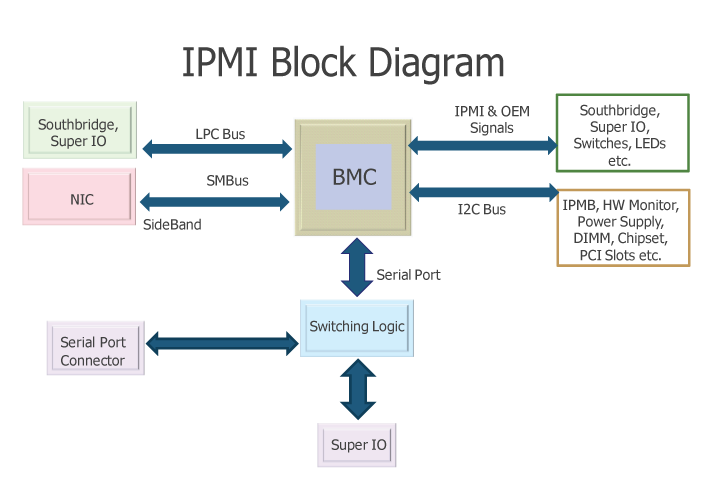
\includegraphics[scale=0.35]{ipmi-block-diagram.png}
   	   \end{center}
   \end{frame}

  \subsection{Demo: WebIF and IPMI}
  \begin{frame}{Demo 1}
	  Web interface:  AVR, VirtualMedia, remote boot

	  \begin{block}{Scenario 1: AVR, show boot settings}
		  AVR: show Windows, Start LCM Custom Image, AVR: Show Linux
	  \end{block}
	  \pause

	  \begin{block}{Scenario 2: IPMI - via ipmitool}

		  \small{\$ ipmitool -U admin -P admin -H 192.168.1.1 -I lanplus [command line]} \newline

		  command line variants:
		  \begin{itemize}
			  \item chassis status
			  \item lan print
			  \item user list
			  \item sensor	
		  \end{itemize}

	  \end{block}

  \end{frame}

\section{Road to Linux: from iRMC S1/ThreadX to iRMC S4/Linux}
  \subsection{Early days - ThreadX : S1 - S2/S3}
  \begin{frame}{iRMC S1 - S2/S3 OS}
	  \begin{center}
		  
\includegraphics[width=0.8\textwidth]{logo/threadx.jpg}
	  \end{center}
	  \begin{block}{Pro}
		  \begin{itemize}
			  \item Advanced Real-Time Operation System
			  \item Small footprint
			  \item Fast performance
		  \end{itemize}
	  \end{block}
	  \pause
	  
	  \begin{block}{Contra}
		  \begin{itemize}
			  \item Lack of available developers
			  \item Lack of 3rd party ready components
			  \item High cost of support
			  \item Long features time-to-market
			  \item Environment compatible only with themselves
		  \end{itemize}
	  \end{block}

  \end{frame}
  \subsection{Migration to Linux: S4}
  \begin{frame}{Why Linux}
	  
\includegraphics[scale=0.4]{dont-fear-the-penguins.jpg}
	  \pause

	  \alert{Cost of development and support}
	  \begin{itemize}
		  \item More developers available
		  \item Huge amount of 3rd party ready components
		  \item Faster development
		  \item HW platform fast enough to run it
	  \end{itemize}

  \end{frame}
  \begin{frame}{Main challenges}

	  \begin{block}{Backward compatibility}

		\begin{columns}[onlytextwidth]
			\begin{column}{0.6\textwidth}
				\begin{itemize}
					\item Same interfaces (UI, protocols) 
					\item Binary firmware upgrades
				\end{itemize}
			\end{column}

			\begin{column}{0.4\textwidth}
				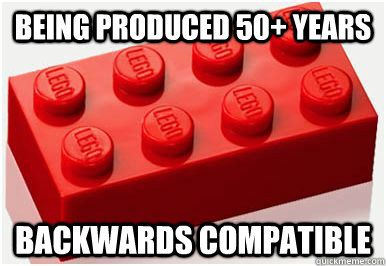
\includegraphics[width=\textwidth]{backward-compat.jpg}
			\end{column}
		\end{columns}
	  \end{block}
	  \pause

	  \begin{block}{Code re-use}

		  \begin{columns}[onlytextwidth]
		  	\begin{column}{0.3\textwidth}
			      	
\includegraphics[width=\textwidth]{code-reuse.jpg}
			\end{column}

			\begin{column}{0.7\textwidth}
				\begin{itemize}
					\item OS API are different
					\item OS layout completely different
					\item HW-related stuff to rewrite from scratch
				\end{itemize}
			\end{column}
		\end{columns}
	  \end{block}

  \end{frame}

  \subsection{Demo: RemoteManager - bug-to-bug compatible}
  \begin{frame}{Demo 2: OpenSSH + RemoteManager}
	  \alert{Interface \st{bug to bug} byte to byte identical to ThreadX}.

	  \begin{center}
		  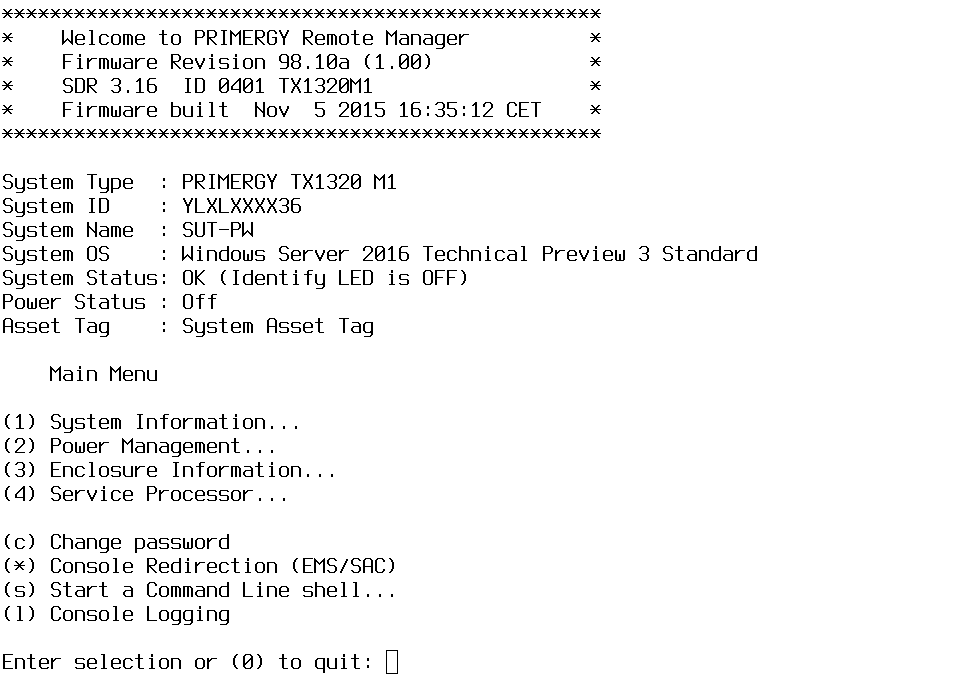
\includegraphics[width=0.8\textwidth]{screenshot/remote-manager.png}
	  \end{center}

  \end{frame}

\section{Linux based firmware}
  \subsection{Components}
  \begin{frame}{iRMC Firmware components}

	  \begin{block}{Free and Open Source Software}
		\begin{columns}[onlytextwidth]
			\begin{column}{0.6\textwidth}
			      	\begin{itemize}
					\item Linux Kernel
					\item U-Boot bootloader
					\item Busybox
					\item GNU Glibc
					\item Net-SNMP
					\item OpenSSH
				\end{itemize}
			\end{column}

			\begin{column}{0.3\textwidth}

				
\includegraphics[width=0.5\textwidth]{logo/linux.jpg} 			
				
\includegraphics[width=0.5\textwidth]{logo/busybox.png}
				
				
\includegraphics[width=0.5\textwidth]{logo/openssl.png} 
				
\includegraphics[width=0.5\textwidth]{logo/netsnmp.jpg}

				
\includegraphics[width=0.5\textwidth]{logo/openssh.png} 
				
\includegraphics[width=0.5\textwidth]{logo/gnu.png}


			\end{column}
		\end{columns}
				
	  \end{block}
	  \pause

	  \begin{block}{Closed source}

		\begin{columns}[onlytextwidth]
			\begin{column}{0.3\textwidth}
				\begin{center}
					
\includegraphics[width=\textwidth]{logo/proprietary-software.jpg}
				\end{center}
			\end{column}
			\begin{column}{0.6\textwidth}
				\begin{itemize}
					\item IPMI full stack powered by AMI MegaRAC
					\item WebServer 
					\item SNMP agents
				\end{itemize}
			\end{column}
		\end{columns}
	  \end{block}
  \end{frame}

  \begin{frame}{iRMC firmware internals}
	
	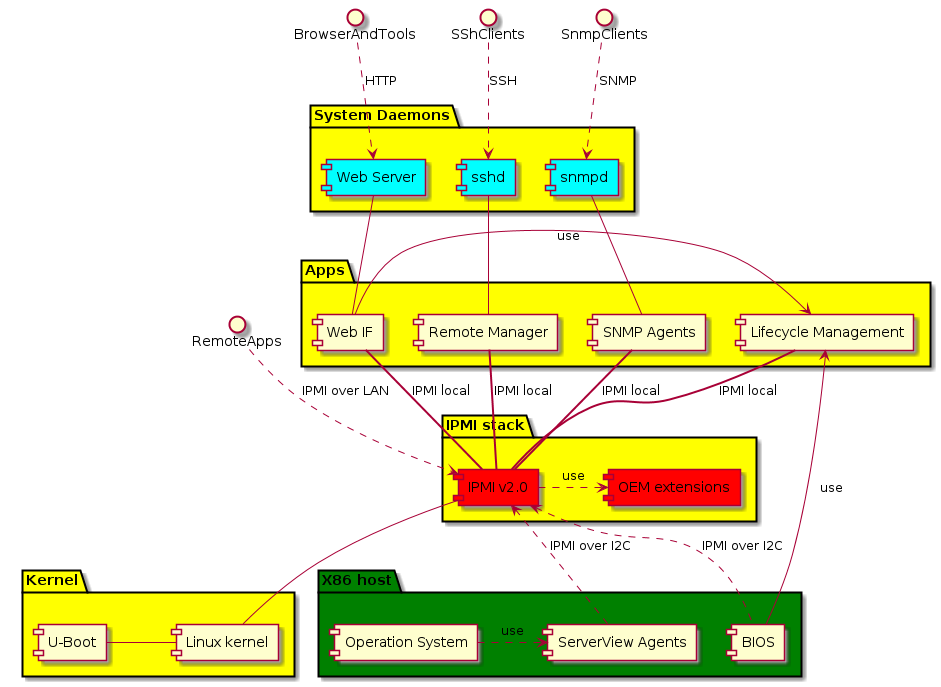
\includegraphics[width=\textwidth]{diagrams/irmc-components.png}

  \end{frame}

  \subsection{Develoment environment}

  \begin{frame}{Development environment}
	  \begin{block}{LXC containers + X2go for developers}
		  The same environment for all to build and debug.

		  Read-only root filesystem on container.

		  Debian GNU/Linux based.
	  \end{block}
	  
	  \begin{block}{Custom package system by AMI MegaRAC technology}
		  Used only in development and build process.

		  Not used for updates.

		  Package format similar to DEB, but not the same.
	  \end{block}

	  \begin{block}{Eclipse-based IDE + AMI MegaRAC extensions}
		  Rich IDE + version control + packaging system integration
	  \end{block}
	  
	  
\includegraphics[height=30pt,width=30pt]{logo/subversion.png}
	  
\includegraphics[height=30pt]{logo/debian.png}
	  
\includegraphics[height=40pt]{logo/x2go-logo.png}
	  
\includegraphics[height=30pt]{logo/lxc.png}
	  
\includegraphics[height=40pt]{logo/megarac-development-studio.png}

  \end{frame}

  \begin{frame}{IDE: Eclipse + AMI MegaRAC extensions}
	  \begin{center}
		  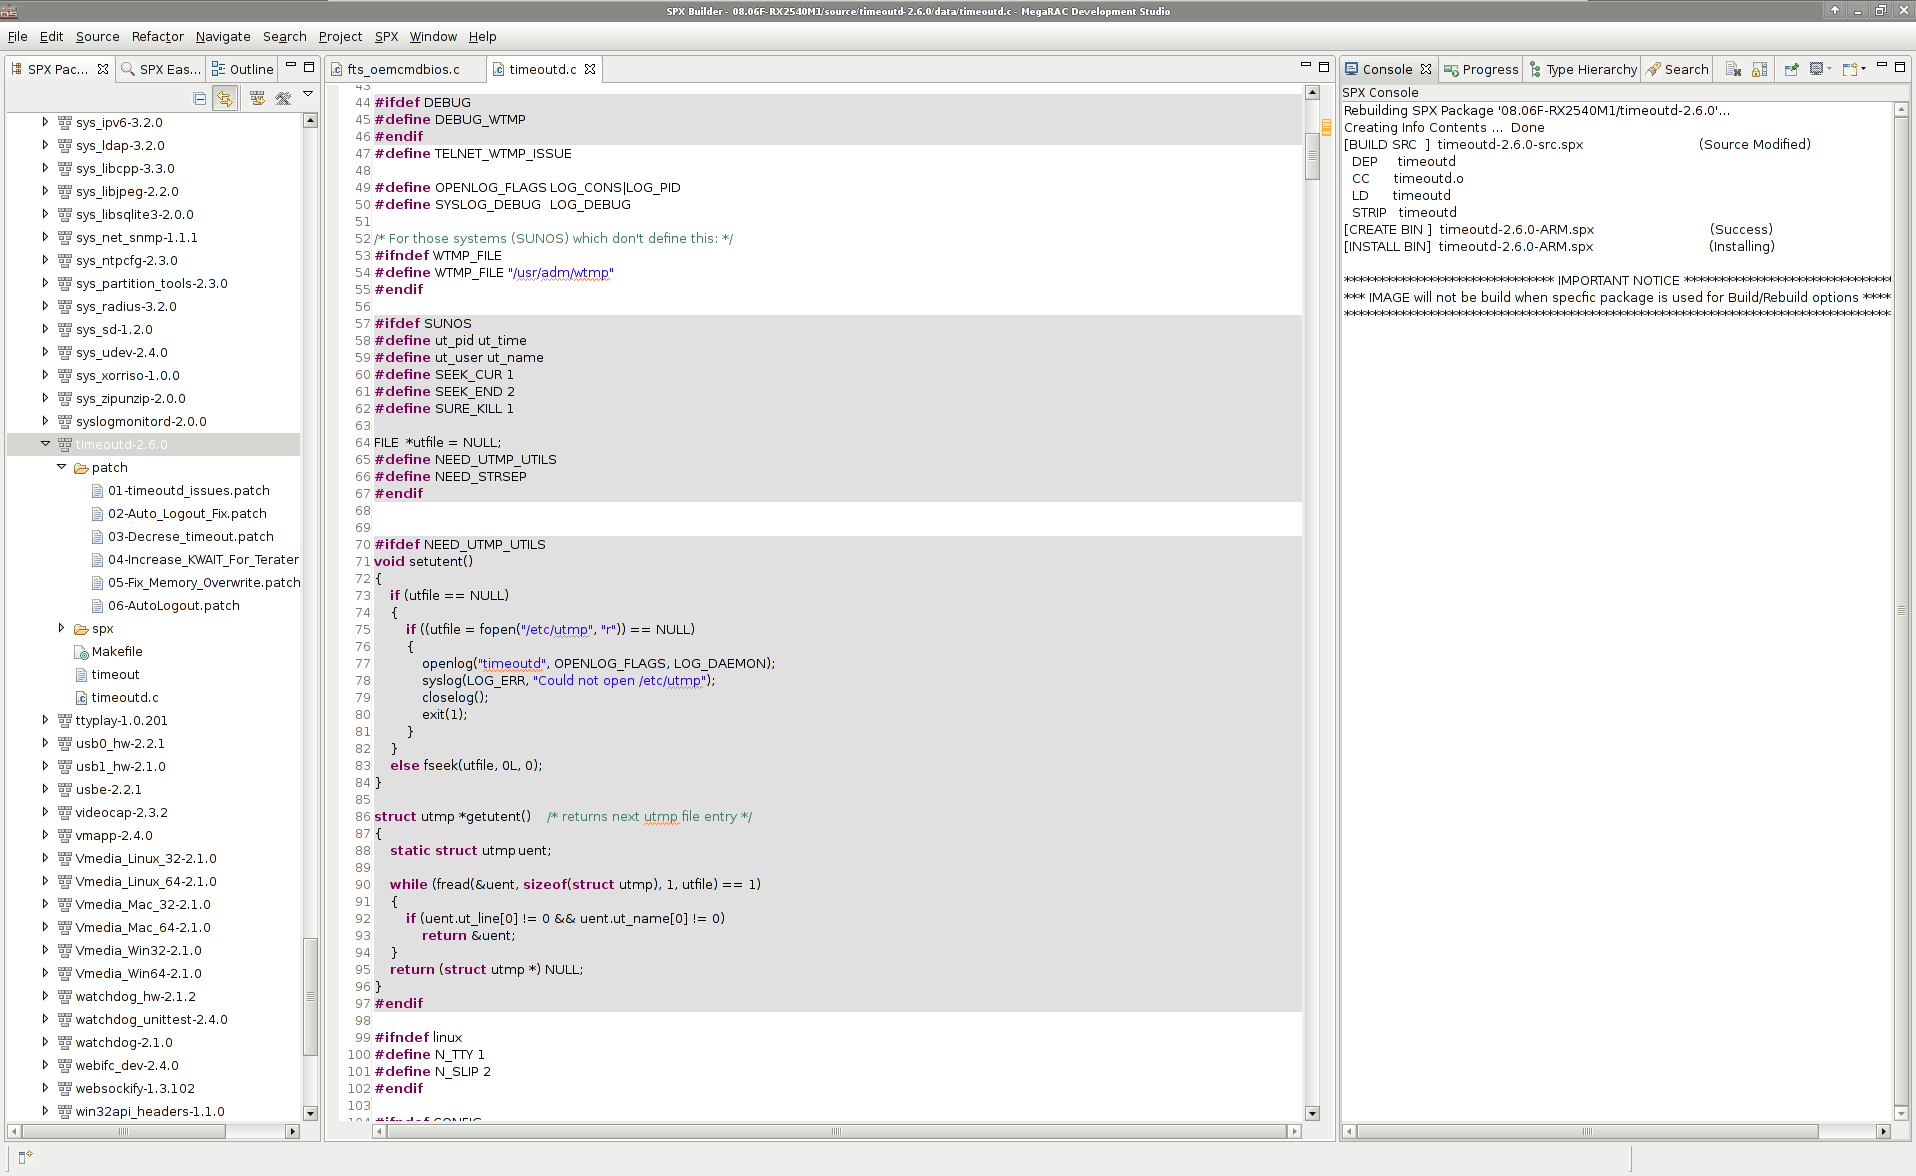
\includegraphics[width=250pt]{screenshot/ide-screenshot.png}
	  \end{center}
	  
\includegraphics[height=30pt]{logo/eclipse-mp-built.png}
	  
\includegraphics[height=40pt]{logo/megarac-development-studio.png}
  \end{frame}
  

  \begin{frame}{Development cycle}

	  \begin{center}
		  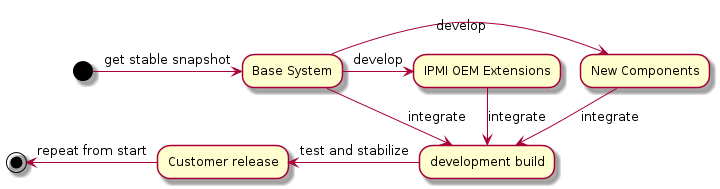
\includegraphics[height=80pt]{diagrams/embedded-release-cycle.png}
	  \end{center}

	  Very typical Embedded Linux development cycle (simplified view):
	  \begin{enumerate}
		  \item Get base system snapshot and freeze it
		  \item Develop new components and IPMI OEM extensions
		  \item Bug fix and stabilization
		  \item Test it hard
		  \item Release firmware to customers
		  \item Repeat once again from step  (1).
	  \end{enumerate}
  \end{frame}

  \subsection{FOSS legal questions}
  \begin{frame}{FOSS legal questions}
	  \begin{itemize}
		  \item Following the FOSS licenses
		  \item Special policy for FOSS components using
		  \item Consolidation of components legal status
		  \item Rare upstream communication \footnote{no significant changes in upstream}
		  \item FOSS component sources - by demand from support
	  \end{itemize}
  \end{frame}

  \subsection{Demo: inside the Linux on iRMC}
  \begin{frame}{Demo 3}
	 Development login via SSH.

	 Show typical Embedded Linux system.
  \end{frame}



\section*{Summary}
\begin{frame}{Questions? Remarks?}
  
  \begin{center}
    \pgfuseimage{fujitsu-shaping}
  \end{center}

  \begin{itemize}
	  \item \tiny{Fujitsu Primergy servers: http://www.fujitsu.com/fts/products/computing/servers/primergy/ }
	  \item \tiny{iRMC S4 manual: http://manuals.ts.fujitsu.com/file/11470/irmc-s4-ug-en.pdf}
	  \item \tiny{Emulex Pilot 3 iBMC specs: http://www.emulex.com/products/controllers/management-controllers/pilot-baseboard-management-controller/specifications}
	  \item \tiny{AMI MegaRAC technology by American Megatrends Inc: http://ami.com/products/remote-management/}
	  \item \tiny{ThreadX RTOS: http://rtos.com/products/threadx }
	  \item \tiny{Fujitsu Technology Solutions: http://www.fujitsu.com/fts}
	\end{itemize}

  contact: Vladimir.Shakhov at ts.fujitsu.com


\end{frame}

\end{document}
